% Drawing 77/05-1 -- folder 77, batch 05, archive page 83 (PDF page 84).
% Transcription: en tête de page, un schéma de traits obliques et de courbes, portant les inscriptions « dans $\Delta^{\nu}$ \struck{$A^{*}$} », « $\partial\in A^{*}$ », « $\Delta\notin A^{*}$ », « \ill{} » ; l'ensemble est barré.
% Kind: struck schema of oblique strokes and curves with inscriptions. Method 2 (schematic redraw from the facsimile). Status: partial.
% Notes: At the head of the page, struck as a whole: oblique strokes and large arcs over a base line, a partial box, and the inscriptions "dans Delta^nu A^*" (A^* struck), "d in A^*" (read 2 in A^* on the crop), "Delta notin A^*", and an illegible group (a ringed letter) left out. Strokes are approximate.
% Coordinates: 1 unit = 1 mm = 1/100 of the crop width (bbox in page fractions: [0.15, 0.05, 0.72, 0.2]).
% Redrawn by Claude (claude-opus-5-5), issue #73, 2026-11-07; not checked by a human; not compiled (no TeX in the session).
% Rights: reproduces part of the work -- behind RENDER_TRANSCRIPTS, never published by itself.
\documentclass[tikz,border=3pt]{standalone}
\usepackage{amsmath,amssymb}
\usetikzlibrary{patterns,arrows.meta}
\tikzset{pencil/.style={black!45}, struck/.style={black!35}, mark/.style={circle,draw,inner sep=1.3pt}, pt/.style={circle,fill,inner sep=0.9pt}, opt/.style={circle,draw,fill=white,inner sep=1.1pt}}
\begin{document}
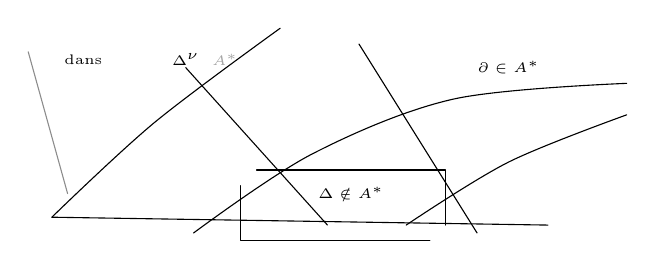
\begin{tikzpicture}[x=1mm,y=1mm,line cap=round,line join=round,font=\scriptsize]
\draw[pencil] (24,-11) -- (29,-29);
\draw plot[smooth, tension=0.55] coordinates {(27,-32) (40,-20) (56,-8)};
\draw (44,-13) -- (62,-33);
\draw (66,-10) -- (81,-34);
\draw plot[smooth, tension=0.55] coordinates {(45,-34) (60,-24) (78,-17) (100,-15)};
\draw plot[smooth, tension=0.55] coordinates {(72,-33) (85,-25) (100,-19)};
\draw (27,-32) -- (90,-33);
\draw (53,-26) -- (77,-26) -- (77,-33);
\draw (51,-28) -- (51,-35) -- (75,-35);
\node[inner sep=1pt] at (31,-12) {\tiny dans};
\node[inner sep=1pt] at (44,-12) {\tiny $\Delta^\nu$};
\node[inner sep=1pt,struck] at (49,-12) {\tiny $A^*$};
\node[inner sep=1pt] at (85,-13) {\tiny $\partial\in A^*$};
\node[inner sep=1pt] at (65,-29) {\tiny $\Delta\notin A^*$};
\end{tikzpicture}
\end{document}
